\documentclass[11pt, a4paper]{article}

%Packages
\usepackage[utf8]{inputenc}
\usepackage{textcomp}
\usepackage[spanish, es-tabla]{babel}
\renewcommand*\familydefault{\sfdefault} 		% Sans Serif as default font


\usepackage{amsmath}
\usepackage{amsfonts}
\usepackage{amssymb}
\usepackage{float}
\usepackage{graphicx}
\usepackage{bm}



\graphicspath{ {./Imagenes/} }

\usepackage{multirow}
\setlength{\headheight}{14pt}
\setlength{\doublerulesep}{\arrayrulewidth}

\usepackage{array}
\newcolumntype{C}[1]{>{\centering\let\newline\\\arraybackslash\hspace{0pt}}m{#1}}

\usepackage[american, nooldvoltagedirection]{circuitikz}

\usepackage{fancyhdr}


\usepackage{units} 
\usepackage{tikz}
\usetikzlibrary{arrows.meta}
\usetikzlibrary{babel,positioning}


\pagestyle{fancy}
\fancyhf{}
\lhead{22.42 Laboratorio de Electrónica}


%\rhead{Bertachini, Lambertucci, Londero, Mechoulam}
\rfoot{Página \thepage}

\usepackage{hyperref}



\begin{document}

%%%%%%%%%%%%%%%%%%%%%%%%%%%%%%%%%%%%%%%%%%%%%%%%%%%%%%%%%%%%%%%%%%%%%%%%% 
%								CARATULA								%
%%%%%%%%%%%%%%%%%%%%%%%%%%%%%%%%%%%%%%%%%%%%%%%%%%%%%%%%%%%%%%%%%%%%%%%%% 

\begin{titlepage}

\newcommand{\HRule}{\rule{\linewidth}{0.5mm}}
\center
\mbox{\textsc{\large \bfseries {INSTITUTO TECNOLÓGICO DE BUENOS AIRES}}}\\[1cm]
\textsc{\Large 22.42 Laboratorio de Electrónica}\\[0.5cm]


\HRule \\[0.6cm]
{ \Huge \bfseries Trabajo Práctico N$^{\circ}$4}\\[0.4cm] 
\HRule \\[1.5cm]


{\large

\emph{Grupo 3}\\
\vspace{3px}

\begin{tabular}{lr} 	
\textsc{Bertachini}, Germán  & 58750 \\ 	
\textsc{Lambertucci}, Guido Enrique  & 58009 \\
\textsc{Londero Bonaparte}, Tomás Guillermo  & 58150 \\
\textsc{Mechoulam}, Alan  &  58438\\
\textsc{Scapolla}, Franco & 58465
\end{tabular}

\vspace{20px}

\emph{Profesores}\\
\vspace{3px}
\textsc{Cossutta}, Pablo Martín\\
\textsc{Weill}, María\\
\textsc{Salvati}, Matías\\	
\vspace{100px}

\begin{tabular}{ll}

Presentado: & 15/10/19\\

\end{tabular}

}

\vfill

\end{titlepage}



%%%%%%%%%%%%%%%%%%%%%%%%%%%%%%%%%%%%%%%%%%%%%%%%%%%%%%%%%%%%%%%%%%%%%%%%% 
%								INFORME									%
%%%%%%%%%%%%%%%%%%%%%%%%%%%%%%%%%%%%%%%%%%%%%%%%%%%%%%%%%%%%%%%%%%%%%%%%%


%%%%%%%%%%%%%%%%%%%%%%%%%%%%%%%%%%%%%%%%%%%%%%%%%%%%%%%%%%%%%%%%%%%%%%%%% 
%					RECORTAR IMAGEN DEL OSCILOSCOPIO					%
%%%%%%%%%%%%%%%%%%%%%%%%%%%%%%%%%%%%%%%%%%%%%%%%%%%%%%%%%%%%%%%%%%%%%%%%%

%\begin{figure}[H]
%	\centering
%	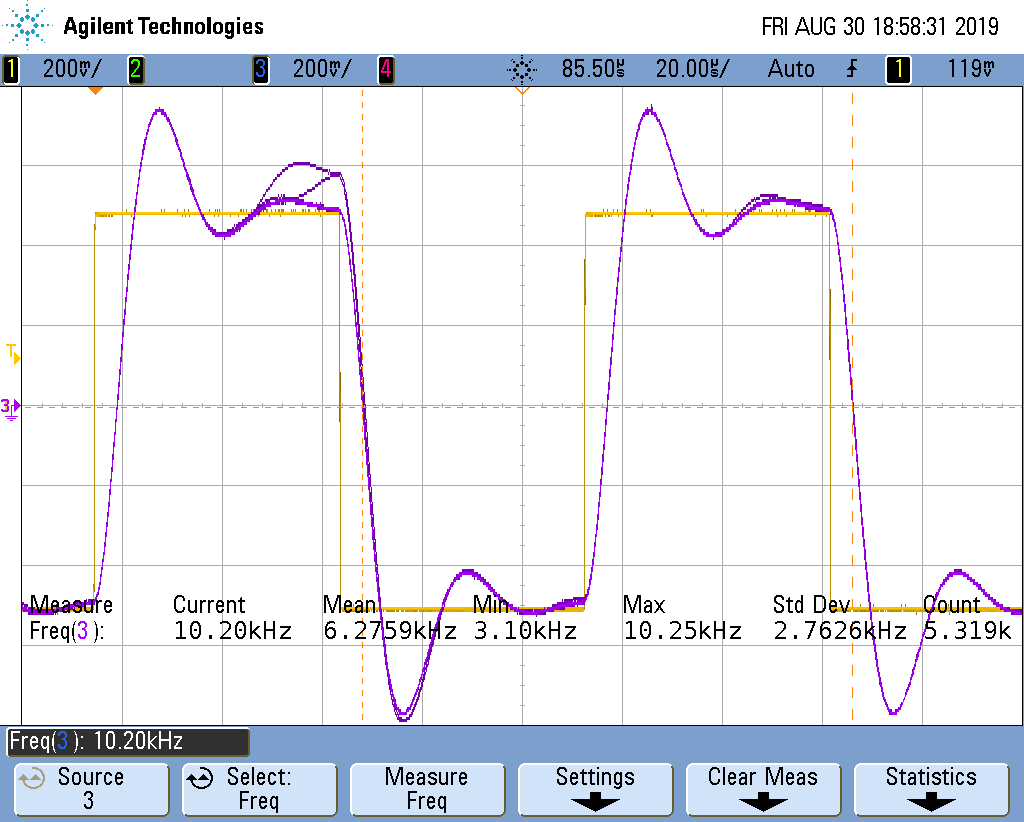
\includegraphics[width=0.9\textwidth , trim={0.7cm 6.25cm  0 3.5cm},clip]{scope_1}
%	%trim={<left> <lower> <right> <upper>}
%\caption{...}
%	\label{fig:...}
%\end{figure}


\section*{Introducción}

En el siguiente informe se realizan diversas mediciones con el osciloscopio, con el objetivo de mejorar el manejo y comprensión de dicho instrumento.

\section*{Desarrollo de la Experiencia}

\subsection*{Filtro Pasa-bajos de Primer Orden}
Se realiza en un protoboard el circuito mostrado en la figura (\ref{figure:circuito_Pasa_bajos}). Para esto se utilizó una resistencia $ R = 3,9 \ K\Omega $ y un capacitor $ C = 2,2 \ nF $. Además, se utilizó el analizador de impedancia con ambos componentes para medir sus valores reales obteniendose los valores expresados en la tabla (\ref{table:valores_calculados1}) .
%Circuito pasabajo
	\begin{figure}[ht]
	\centering
  \begin{circuitikz}[scale=1.6]\draw
	(0,2) to[V, l=$V_{inp}$,a=$10 V_{pp}$,*-*] (0,0)
	(0,2) to[R, i=i(t), v=$V_r$,l=$R$,,*-*] (4,2)
	(4,2) to[C, v=$V_c$,l=$C$, *-*] (4,0)
	(0,0) -- (4,0)

	(2,0) node[ground] {}
	(2,0) node[circ]{}
	(0,2) node[circ]{}

 	{[anchor=south east]  (0,2) node {A} (4,2) node {B} (4,0) node {C} };
 	\end{circuitikz}

 \caption{Filtro Pasa-bajos}
\label{figure:circuito_Pasa_bajos} 
   \end{figure}
 %~Circuito pasabajo
\par
Primeramente, se calculó la frecuencia de corte teórica tomando como referencia los valores de referencia de los componentes, dando como resultado una frecuencia de $18,55 KHz$. Por otro lado, con la fuente se aplicó una tensión senoidal de una amplitud de $9,81 V$ para determinar la frecuencia de corte real de dicho circuito, obteniéndose así una frecuencia de $18,44 KHz$ detectada por ser la frecuencia a la que se produce un desfasaje de 45° entre la señal de entrada y de salida. \par Consecuentemente, conocida la frecuencia de corte real del circuito se procede a calcular el valor de capacitancia para la nueva frecuencia de corte, tomando como valor del resistor primero el teórico ($R_T$) y luego el medido por el analizador de impedancia ($R_M$). Dichos valores se ven expresados en la siguiente tabla:

%% Valores obtenidos
 \begin{center}
     \begin{table}[H]
     \centering
	 \renewcommand{\arraystretch}{1.1}
         \begin{tabular}{c c c c c c}
            \hline 
            $\bm{|V|}$ &  $\bm{|V_C|}$ & $\bm{R}$ &  $\bm{C_{calculado}}$ &    $\bm{C_{medido}}$   &  $\bm{Error}$\\ \hline
            $9.81V$& $6.84V$ & $R_T = 3k90\Omega$  & $2.2126nF$ & $2.238nF$ & $1.13\%$ \\  
            $9.81V$& $6.84V$ & $R_M = 3k87\Omega$ & $2.2297nF$ & $2.238nF$ & $0.37 \%$ \\   \hline
        \end{tabular}
        \caption{Valores obtenidos}
        \label{table:valores_calculados1}
    \end{table}
\end{center}
%% ~Valores obtenidos
A continuación, se mide la diferencia de fase entre la corriente y la tensión en el capacitor, y se verifica la suma vectorial de las tensiones, es decir $ \overrightarrow{V} = \overrightarrow{V_R} \ + \ \overrightarrow{V_C} $.\par
Al ser $\overrightarrow{i}$ coplanar con $\overrightarrow{V_r}$ podemos medir la diferencia de fase entre ambas tensiones y encontraremos la diferencia entre $\overrightarrow{i}$ y $\overrightarrow{V_C}$. La diferencia de fase será siempre de $90^\circ$ ya que la caída de tensión en la resistencia será puramente real y la caída de tensión en el capacitor será puramente imaginaria  como se puede ver en el siguiente diagrama:

\begin{figure}[ht]
	\centering
	\begin{tikzpicture}[scale=0.6]{>=Stealth}
	\draw[black,thick,<->] (-4,0) -- (4,0) node[anchor=north west]{Im};
	\draw[black,thick,<->] (0,-4) -- (0,4) node[anchor=south east]{Re};
	\draw[black,thick] (0.5,0) -- (0.5,-0.5) -- (0,-0.5) ;
	\draw[blue,ultra thick,->,-Latex] (0,0) -- (3,0) node[anchor=south east]{$\overrightarrow{V_r}$};
	\draw[red,ultra thick,->>,-Latex] (0,0) -- (2,0) node[anchor=south east]{$\overrightarrow{i}$};
	\draw[blue,ultra thick,->>,-Latex] (0,0) -- (0,-3) node[anchor=south east]{$\overrightarrow{V_c}$};
	\draw[blue,ultra thick,->>,-Latex] (0,-3) -- (3,0) node[anchor=north west]{$\overrightarrow{V}$};
	\draw[help lines,step=1cm,gray,thin] (-3.9,-3.9) grid (3.9,3.9);
	\end{tikzpicture}
	\caption{Diagrama vectorial de las tensiones}
	\label{figure:Diagrama_vectorial}
\end{figure}

Esto se puede apreciar claramente en la captura de la pantalla del osciloscopio ({\ref{figure:VrvsVs}}), donde la señal verde representa $\overrightarrow{V_R}$ (coplanar con$\overrightarrow{i}$), la señal amarilla $\overrightarrow{V}$ y la señal violeta $\overrightarrow{V_c}$. La captura se realizó trabajando sobre la frecuencia de corte por lo que se puede apreciar como claramente el desfasaje es de $45^\circ$ entre ambas tensiones ($\overrightarrow{V_R}$ y $\overrightarrow{V}$) y los módulos, por ende se representa la situación planteada en el dibujo ({\ref{figure:Diagrama_vectorial}}).

 \begin{figure}[H]
	\centering
	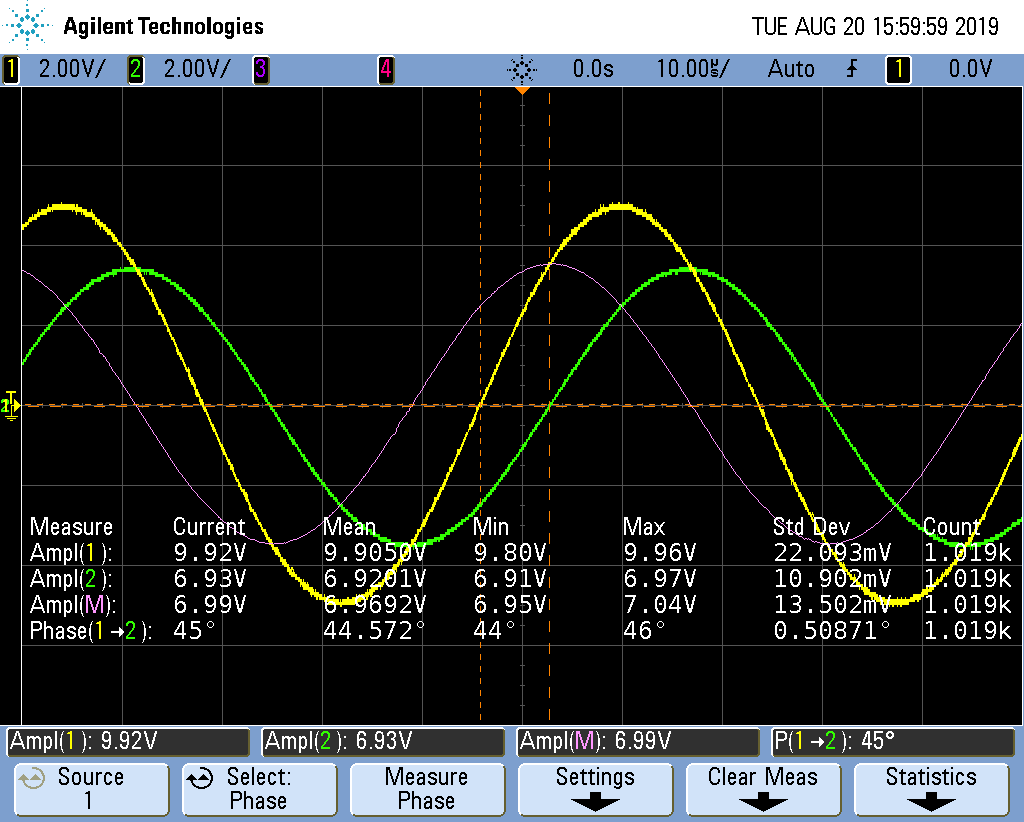
\includegraphics[width=0.8\textwidth,trim={0.7cm 6.25cm  0 3.5cm},clip]{VrvsVvsVc.png}
	\caption{Relación de tensiones}
	\label{figure:VrvsVs}
\end{figure}


\par

Posteriormente, se calcula analíticamente la transferencia del circuito, llegán\-dose a la expresión:

\begin{equation}
	H \left(\$ \right) = \frac{V_C}{V} = \frac{1}{\$CR + 1} = \frac{1}{S \cdot 8.58 \cdot 10^{-6} + 1}
	\label{equ:transfpasabajos}
\end{equation} \\
Además, partiendo de una frecuencia de $10  Hz$ hasta llegar a $1  MHz$, se toman varios valores tanto de la $V_C$ como de $V$, presentados en la tabla (\ref{table:Filtro_pasabajos}). De esta forma, se grafica punto a punto la transferencia y se la compara con la teórica hallada usando la ecuación (\ref{equ:transfpasabajos}), obteniendo los siguientes diagramas de Bode:

\begin{figure}[H]
	\centering
	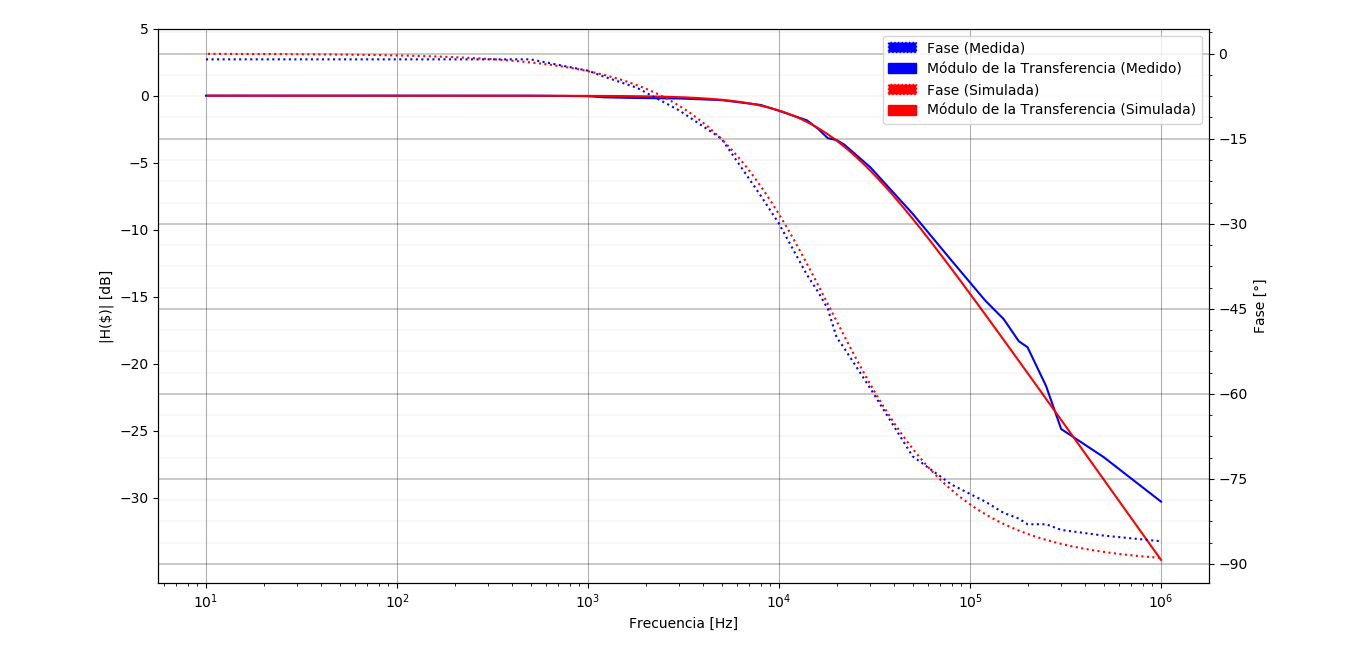
\includegraphics[width=0.9\textwidth]{Bode_filtro_pasabajo.png}
	\caption{Diagramas de Bode - Medido vs Simulado} 
	\label{graf:bodes_pasabajo}
\end{figure}

%%bode RC amplitud y fase (teórico y práctico)

%% Valores obtenidos Bode pasabajos
 \begin{center}
     \begin{table}[H]
     \centering
     \renewcommand{\arraystretch}{1.1}
         \begin{tabular}{ c c c c c c c c }
            \hline 
             \bm{$Medici\acute{o}n$} &  $\bm{|V|}$ & $\bm{|V_c|}$& $\bm{|V_R|}$ & $\bm{f}$ & $\bm{\frac{V_c}{V}[dB]}$ & $\bm{\theta_{\Delta t}}$  &  $\bm{\theta_{XY}}$\\
             \hline
                1&	9.94&	9.94&	0	&	10	&	0.00&	1°&		0.00°\\
				2&	9.81&	9.81&	0	&	500	&	0.00&	1°&		1.24°\\
				3&	9.81&	9.77&	0.04&	1000&	0.04&	3°&		2.60°\\
				4&	9.81&	9.68&	0.13&	1200&	0.12&	4°&		3.24°\\
				5&	9.81&	9.62&	0.19&	1800&	0.17&	6°&		5.13°\\
				6&	9.81&	9.58&	0.23&	3000&	0.21&	10°&	9.09°\\
				7&	9.81&	9.44&	0.37&	5000&	0.33&	15°&	15.73°\\
				8&	9.81&	9.06&	0.75&	8000&	0.69&	25°&	23.74°\\
				9&	9.81&	8.61&	1.20&	10000&	1.13&	30°&	27.90°\\
				10&	9.81&	7.94&	1.87&	14000&	1.84&	39°&	32.01°\\
				11&	9.81&	7.38&	2.43&	16000&	2.47&	42°&	38.45°\\
				12&	9.81&	6.81&	3.00&	18000&	3.17&	45°&	40.95°\\
				13&	9.81&	6.70&	3.11&	20000&	3.31&	50°&	42.60°\\
				14&	9.81&	6.44&	3.37&	22000&	3.66&	52°&	43.88°\\
				15&	9.81&	5.31&	4.50&	30000&	5.33&	59°&	46.20°\\
				16&	9.81&	3.56&	6.25&	50000&	8.80&	71°&	65.83°\\
				17&	9.81&	2.38&	7.43&	80000&	12.30&	76°&	70.55°\\
				18&	9.81&	1.69&	8.12&	120000&	15.28&	79°&	76.28°\\
				19&	9.81&	1.44&	8.37&	150000&	16.67&	81°&	78.12°\\
				20&	9.81&	1.19&	8.62&	180000&	18.32&	82°&	78.41°\\
				21&	9.81&	1.13&	8.68&	200000&	18.77&	83°&	78.41°\\
				22&	9.81&	0.44&	9.37&	250000&	26.96&	83°&	78.41°\\
				23&	9.81&	0.81&	9.00&	300000&	21.66&	84°&	78.41°\\
				24&	9.81&	0.56&	9.25&	500000&	24.87&	85°&	78.41°\\
				25&	9.81&	0.30&	9.51&	1000000&30.29&	86°&	78.41°\\


            \hline 
        \end{tabular}
        \caption{H(\$) - Filtro Pasa-bajos}
        \label{table:Filtro_pasabajos}
    \end{table}
\end{center}
%%~Valores obtenidos Bode pasabajos
\subsubsection*{Excitación con onda cuadrada}

Se procede a excitar el circuito con una cuadrada de amplitud $10 V_{pp}$. Se consideran tres frecuencias características que estarán relacionadas con la frecuencia de corte ($f_c$), siendo las mismas $0.1f_c$, $f_c$ y $10f_c$ respectivamente. \par 

Se puede entender a la señal de onda cuadrada como una composición de ondas de alta y baja frecuencia, estando las primeras componiendo los flancos y las segundas componiendo las zonas "llanas". Al excitar el circuito con una señal de $0.1f_c$ como se observa en la captura (\ref{graf:rta_onda_cuadrada_baja_f}), la misma pasará casi sin modificaciones ya que ninguna frecuencia será filtrada. 


\begin{figure}[H]
	\centering
	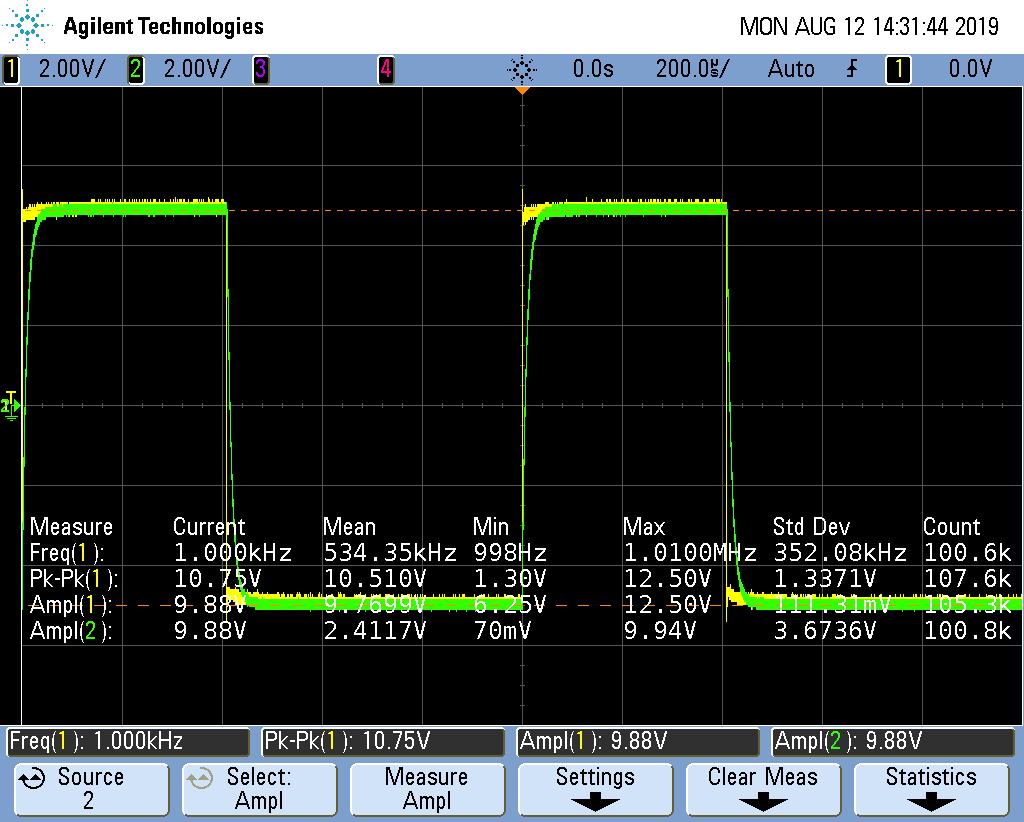
\includegraphics[width=0.8\textwidth,trim={0.5cm 5cm  1 5cm},clip]{rta_onda_cuadrada_baja_f.png}
	\caption{Respuesta del circuito ante señal cuadrada de baja frecuencia} 
	\label{graf:rta_onda_cuadrada_baja_f}
\end{figure}

Al subir a una frecuencia de $f_c$ (\ref{graf:rta_onda_cuadrada_fc}) se verá una deformación de la señal producto de la acción del filtro que se opone a las componentes senoidales de frecuencias altas e integra las de frecuencias bajas.

\begin{figure}[H]
	\centering
	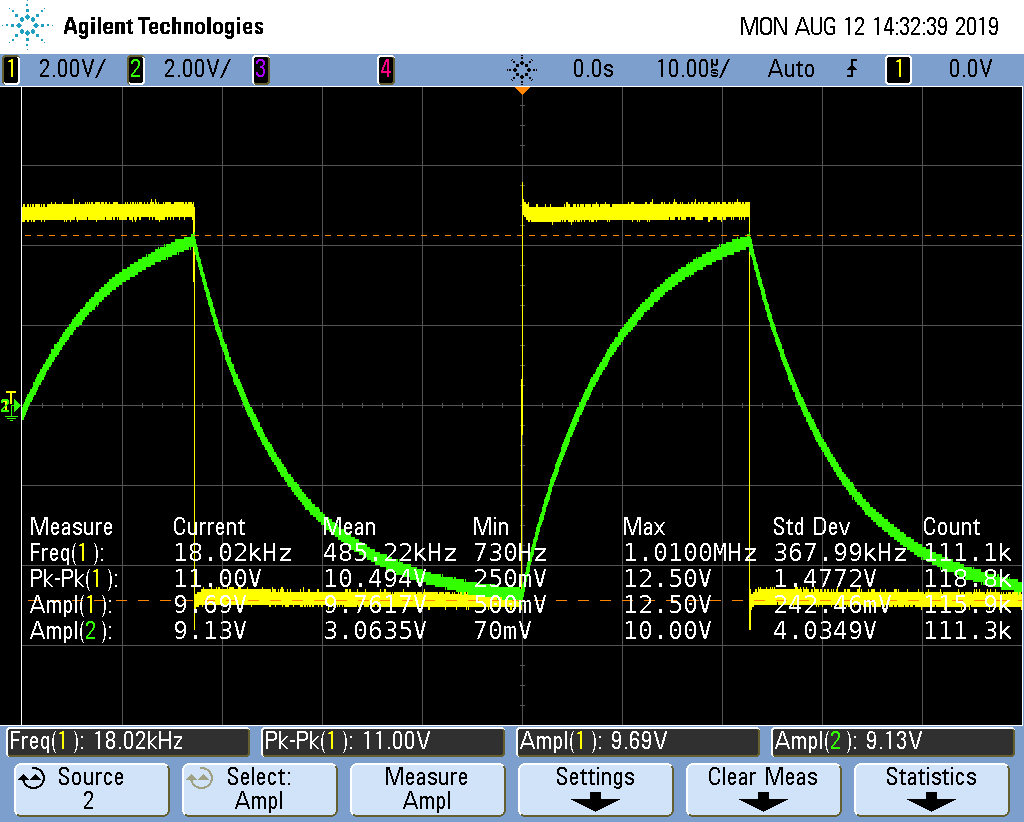
\includegraphics[width=0.8\textwidth,trim={0.5cm 5cm  1 5cm},clip]{rta_onda_cuadrada_fc.png}
	\caption{Respuesta del circuito ante señal cuadrada similar a la frecuencia de corte} 
	\label{graf:rta_onda_cuadrada_fc}
\end{figure}

 A partir de $10f_c$ (\ref{graf:rta_onda_cuadrada_alta_f}), se puede observar claramente el efecto integrador que tiene un filtro pasa-bajo sobre una señal cuadrada, filtrando las señales de alta frecuencia (presentes en los flancos) e integrando las señales de baja frecuencia. Este último hecho se refleja en que dichas ondas se visualizan como constantes a la entrada para luego ser convertidas a una recta a la salida, dando como resultado una señal triangular de amplitud reducida. La demostración analítica se presenta al final de las imágenes.
 
\begin{figure}[H]
	\centering
	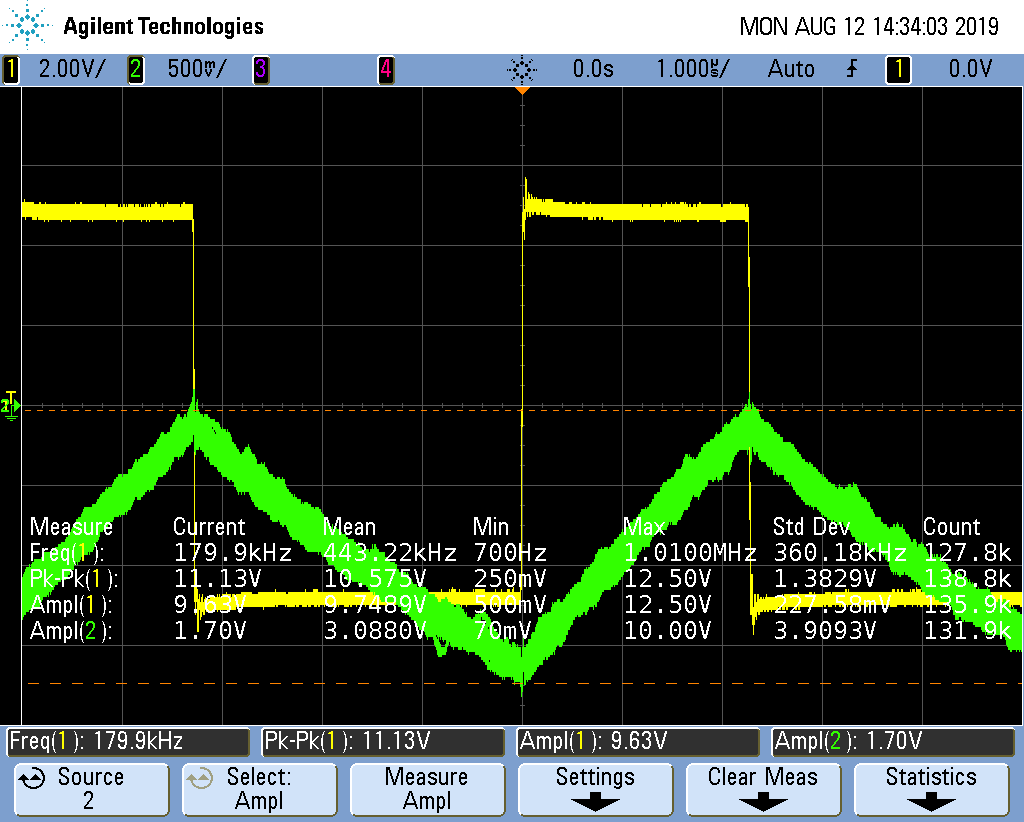
\includegraphics[width=0.8\textwidth,trim={0.5cm 5cm  1 5cm},clip]{rta_onda_cuadrada_alta_f.png}
	\caption{Respuesta del circuito ante señal cuadrada de alta frecuencia} 
	\label{graf:rta_onda_cuadrada_alta_f}
\end{figure}

\subsubsection*{Caída de tensión en la resistencia}

Se calcula $V_R$ como un despeje de la relación entre la tensiones entre $V$ y $V_R$. Se grafica a continuación:

\begin{figure}[H]
	\centering
	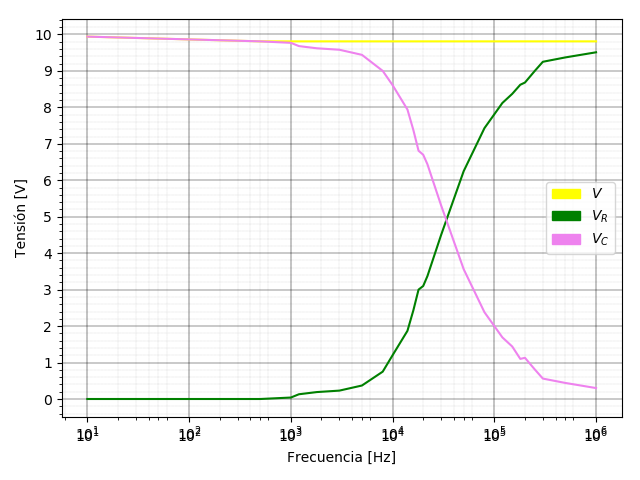
\includegraphics[width=0.7\textwidth]{Tensiones.png}
	\caption{Relación entre las tensiones} 
	\label{graf:Tensiones}
\end{figure}
Se observa claramente como la caída de tensión entre $V_C$ y $V_R$ se complementan para sumar la tensión del generador $V$.


\subsubsection*{Capacitancia residual al medir}

En esta sección del trabajo se investigará como se comporta la capacidad inherente al osciloscopio y sus puntas. 

Primero, se utilizaron las puntas en \textbf{modo x10}. Se calculó la frecuencia de corte presente en dicho circuito considerando que la capactiancia equivalente de las puntas en dicho modo, visto en clase, es de $12 pF$ y tomando como referencia $R_T$. Se obtuvo una frecuencia de corte teórica de $3,40MHz$. \par 
Luego, haciendo uso del analizador de impedancia a esa frecuencia se observó que la capacitancia de las puntas era $15.85 pF$. Por otro lado, se buscó la frecuencia de corte con este último equipo obteniendo una frecuencia de $2.9 MHz$ con una capacitancia asociada de $16.05pF$. Se repite el proceso utilizando la $R_M$. Se llegó a los datos expresados en la siguiente tabla:
%% Valores obtenidos
 \begin{center}
     \begin{table}[ht]
     \centering
	 \renewcommand{\arraystretch}{1.1}
         \begin{tabular}{c c c c c c}
            \hline 
             $\bm{R}$ &  $\bm{C_{calculado}}$ &    $\bm{C_{medido}}$   &  $\bm{Error}$\\ \hline
             $R_T = 3k90\Omega$  & $15.85 pF$ & $16.05 pF$ & $1.24\%$ \\  
             $R_M = 3k87\Omega$ & $16.32 pF$ & $16.20 pF$ & $0.74 \%$ \\   \hline
        \end{tabular}
        \caption{Capacitancia asociada usando una punta en modo x10}
        \label{table:valores_punta_x10}
    \end{table}
\end{center}

%% ~Valores obtenidos
Luego, se utilizaron las puntas en \textbf{modo x1}. Se calculó la frecuencia de corte presente en dicho circuito considerando que la capactiancia equivalente de las puntas en dicho modo, visto en clase, es de $104pF$ y tomando como referencia $R_T$. Se obtuvo una frecuencia de corte teórica de $3,95MHz$. \par Después, haciendo uso del analizador de impedancia a esa frecuencia se observó que la capacitancia de las puntas era $84pF$. Por otro lado, se buscó la frecuencia de corte con este último equipo obteniendo una frecuencia de $6.7MHz$ con una capacitancia asociada de $70pF$. Se repite el proceso utilizando la $R_M$. Se llegó a los datos expresados en la siguiente tabla:
%% Valores obtenidos
 \begin{center}
     \begin{table}[ht]
     \centering
	 \renewcommand{\arraystretch}{1.1}
         \begin{tabular}{ c c c c}
            \hline 
             $\bm{R}$ &  $\bm{C_{calculado}}$ &    $\bm{C_{medido}}$   &  $\bm{Error}$\\ \hline
             $R_T = 3k90\Omega$  & $84 pF$ & $72 pF$ & $16.6\%$ \\  
             $R_M = 3k87\Omega$ & $84.5 pF$ & $71 pF$ & $19 \%$ \\   \hline
        \end{tabular}
        \caption{Capacitancia asociada usando una punta en modo x1}
        \label{table:valores_punta_x1}
    \end{table}
\end{center}
%% ~Valores obtenidos


\subsubsection*{Conclusiones}
Como primera conclusión, se puede observar claramente la diferencia entre los valores teóricos aportados por el fabricante y los valores a los cuales se llega empíricamente en el laboratorio. El principal instrumento que permite visualizar dicha brecha entre lo empírico y lo teórico es el analizador de impedancia ya que nos indica la magnitud real ya sea de resistividad o de capacitancia del componente que está siendo usado. Dicha diferencia se ve reflejada en una reducción significativa del error al hacer uso del valor empírico de la resistencia para el calculo de la capacitancia, obteniendo una reducción del error de 32.74\%. \par
Por otro lado, también debido a las diferencias planteadas anteriormente, la frecuencia de corte del circuito a la que se llegó teóricamente difiere, aunque en baja proporción, de la obtenida al realizar la práctica. 
\par
También, se pudo observar la diferencia entre medir la diferencia de fase usando los métodos $\theta_{\Delta t}$ y $\theta_{XY}$, siendo el primero el método más práctico y eficaz mientras que el segundo requiere de un mayor procedimiento. Sin embargo, el método $\theta_{XY}$ es de gran utilidad para visualizar las relaciones geométricas entre las magnitudes medidas si fuera necesario.
\par

Es necesario mencionar que para ningún cálculo se considera la capacitancia asociada al cable coaxil del generador de funciones ni a las puntas de osciloscopio utilizadas ya que para los valores de capacitancia manejados, dicha capacitancia "residual" se vuelve despreciable por estar varios ordenes de magnitud por debajo. \par
El caso de la capacitancia "residual" tiene su apartado especial en el que se puede observar claramente como la estructura de los instrumentos de medición difiere de tener un carácter ideal, dependiendo la magnitud de su capacitancia según el modo en que se utilizan las puntas. Es indispensable siempre ser consciente de dicho efecto ya que puede afectar gravemente las mediciones ante circuitos donde la capacitancia "residual" no es despreciable respecto de la propia del circuito.
\par
Respecto de los diagramas de Bode, se puede apreciar una gran similitud entre el simulado y el obtenido empíricamente. Se estima que las pequeñas diferencias observadas se deben a la limitada cantidad de puntos obtenidos en el laboratorio en comparación con el mayor muestreo que obtiene un programa como LTSpice al simular dicho circuito.
%algo más?
%Falta agregar algo respecto de Vr que está mal
%Falta agregar algo respecto de lo de la onda cuadrada
\break

\subsection*{Filtro Pasa-altos de Primer Orden}

Con los mismos elementos utilizados para armar el circuito (\ref{figure:circuito_Pasa_bajos}), se elabora el circuito pasa altos (\ref{figure:circuito_pasa_altos}). Su transferencia se calcula analíticamente obteniéndose:

\begin{equation}
	H \left(\$ \right) = \frac{V_C}{V} = \frac{\$CR}{\$CR + 1} = \frac{\$ \cdot 8.58 \cdot 10^{-6}}{S \cdot 8.58 \cdot 10^{-6} + 1}
	\label{equ:transfpasaaltos}
\end{equation}

%Circuito pasaalto
\begin{figure}[H]
  \begin{center}\begin{circuitikz}[scale=1.6]\draw
(0,2) to[V, l=$V_inp$,a=$10 V_{pp}$,*-*] (0,0)
(0,2) to[C, v=$V_c$,l=$C$, *-*] (4,2)
(4,2) to[R, i=i(t), v=$V_r$,l=$R$,,*-*] (4,0)
(0,0) -- (4,0)

(2,0) node[ground] {}
(2,0) node[circ]{}
(0,2) node[circ]{}

 {[anchor=south east]  (0,2) node {A} (4,2) node {B} (4,0) node {C} };\end{circuitikz} 
 
 
 \end{center}
 \caption{Filtro Pasa-altos}
 \label{figure:circuito_pasa_altos}
 \end{figure}
 %~Circuito pasaalto

Al igual que con el filtro pasabajos, se procede a medir varios puntos de la tensión de la resistencia y de la fuente, variando la frecuencia. Así se grafica la transferencia medida y se la compara con la teórica hallada en (\ref{equ:transfpasaaltos}), dando como resultado los siguientes diagramas de Bode:

\begin{figure}[H]
	\centering
	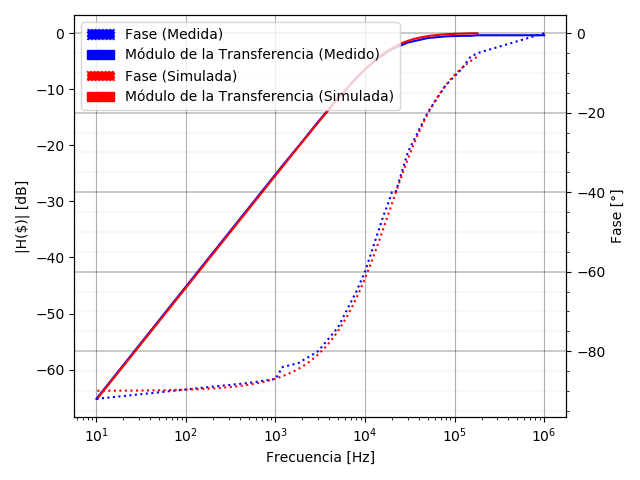
\includegraphics[width=0.9\textwidth]{Bode_filtro_pasaalto.png}
	\caption{Diagramas de Bode - Medido vs Simulado} 
	\label{graf:bodes_pasaalto}
\end{figure}

%% Valores obtenidos Bode pasaltos
 \begin{center}
     \begin{table}[H]
     \centering
	   \renewcommand{\arraystretch}{1.1}
     \label{table:Filtro pasaalto}
         \begin{tabular}{c c c c c c c}
            \hline 
             \bm{$Medici\acute{o}n$}  & $\bm{|V_{in}|}$ & $\bm{|V_c|}$&   $|\bm{V_r|}$ & f&  $\bm{\frac{V_r}{V}[dB]}$ & $\bm{\theta_{\Delta t}}$  \\
             \hline
                1  & 9.94 & 9.865 & 0.075 & 10     & 42.45 & -90° \\
				2  & 9.94 & 9.34  & 0.6   & 500    & 24.38 & -89° \\
				3  & 9.94 & 9.04  & 0.9   & 1000   & 20.86 & -87° \\
				4  & 9.94 & 8.84  & 1.1   & 1200   & 19.12 & -86° \\
				5  & 9.94 & 8.64  & 1.3   & 1800   & 17.67 & -85° \\
				6  & 9.94 & 7.94  & 2     & 3000   & 13.93 & -81° \\
				7  & 9.94 & 6.83  & 3.11  & 5000   & 10.09 & -75° \\
				8  & 9.94 & 5.53  & 4.41  & 8000   & 7.06  & -66° \\
				9  & 9.94 & 5.13  & 4.81  & 10000  & 6.30  & -61° \\
				10 & 9.94 & 3.74  & 6.2   & 14000  & 4.10  & -52° \\
				11 & 9.94 & 3.1   & 6.84  & 16000  & 3.25  & -46° \\
				12 & 9.94 & 3.03  & 6.91  & 18000  & 3.16  & -45° \\
				13 & 9.94 & 2.93  & 7.01  & 20000  & 3.03  & -41° \\
				14 & 9.94 & 2.66  & 7.28  & 22000  & 2.71  & -39° \\
				15 & 9.94 & 1.71  & 8.23  & 30000  & 1.64  & -31° \\
				16 & 9.94 & 1.01  & 8.93  & 50000  & 0.93  & -20° \\
				17 & 9.94 & 0.63  & 9.31  & 80000  & 0.57  & -13° \\
				18 & 9.94 & 0.25  & 9.69  & 120000 & 0.22  & -9°  \\
				19 & 9.94 & 0.23  & 9.71  & 150000 & 0.20  & -6°  \\
				20 & 9.94 & 0.22  & 9.72  & 180000 & 0.19  & -5°  \\
		\hline
        \end{tabular}
        \caption{H(\$) - Filtro Pasa-altos}
    \end{table}
\end{center}

%% ~Valores obtenidos Bode pasaaltos
\subsubsection*{Excitación con onda triangular}

Se procede a excitar el circuito con una triangular de amplitud $10 V_{pp}$. Se consideran tres frecuencias características que estarán relacionadas con la frecuencia de corte ($f_c$), siendo las mismas $0.1f_c$, $f_c$ y $10f_c$ respectivamente. \par 

Se puede entender a la señal de onda traingular como un tipo de señal periódica que presenta unas velocidades de subida y bajada (Slew Rate) constantes. \par Al excitar el circuito con una señal de $0.1f_c$ como se observa en la captura (\ref{graf:rta_onda_triang_baja_f}), se hará presente el efecto derivador que tiene el filtro sobre dicha señal dando como resultado una cuadrada. Esto se debe a que las pendientes de la señal se consideran una recta que al ser derivada dará como resultado una constante.   

\begin{figure}[H]
	\centering
	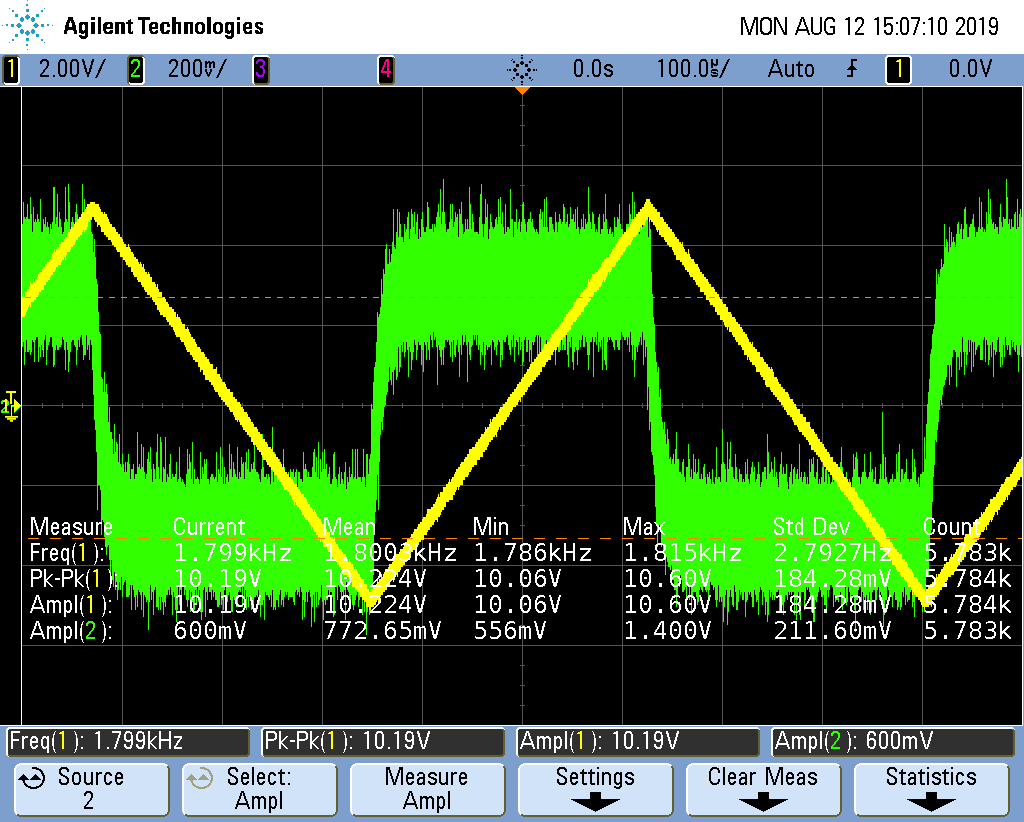
\includegraphics[width=0.8\textwidth,trim={0.5cm 5cm  1 5cm},clip]{rta_onda_triang_baja_f.png}
	\caption{Respuesta del circuito ante señal triangular de baja frecuencia} 
	\label{graf:rta_onda_triang_baja_f}
\end{figure}

Al subir a una frecuencia de $f_c$ (\ref{graf:rta_onda_triang_fc}) se verá una deformación de la señal producto de la acción del filtro que se opone a las frecuencias bajas.

\begin{figure}[H]
	\centering
	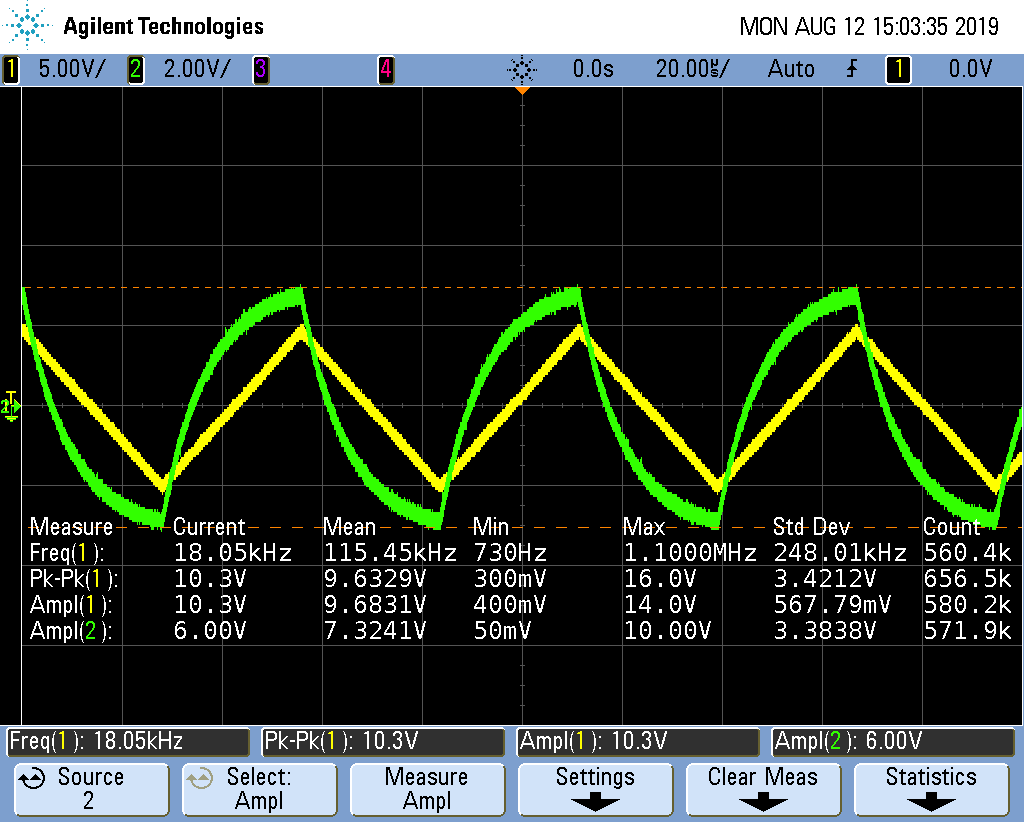
\includegraphics[width=0.8\textwidth,trim={0.5cm 5cm  1 5cm},clip]{rta_onda_triang_fc2.png}
	\caption{Respuesta del circuito ante señal triangular similar a la frecuencia de corte} 
	\label{graf:rta_onda_triang_fc}
\end{figure}

A partir de $10f_c$ (\ref{graf:rta_onda_triang_alta_f}), se puede observar claramente como el filtro deja pasar a toda la señal ya que todas las senoidales que la componen tienen una frecuencia mayor a su $f_c$ dando como resultado una señal a la salida casi idéntica a la original.
La demostración analítica se presenta al final de las imágenes.

\begin{figure}[H]
	\centering
	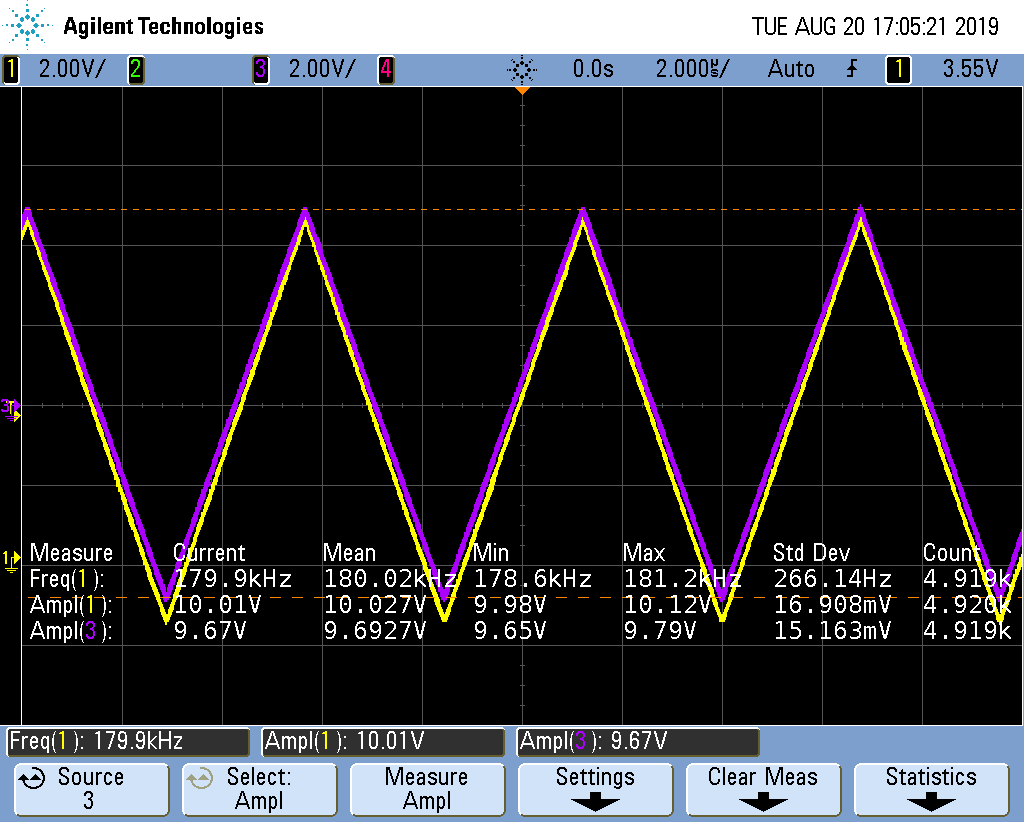
\includegraphics[width=0.8\textwidth,trim={0.5cm 5cm  1 5cm},clip]{rta_onda_triang_alta_f.png}
	\caption{Respuesta del circuito ante señal triangular de alta frecuencia} 
	\label{graf:rta_onda_triang_alta_f}
\end{figure}



\break
\subsection*{Sincronización de Instrumentos}
En este punto se utiliza el barrido automático del generador de funciones, para visualizar en el osciloscopio la respuesta en frecuencia del circuito de la la figura (\ref{figure:circuito_Pasa_bajos}). Se realizó la medición aproximada utilizando dos métodos.

\subsubsection*{Modo XY con dos Generadores}
Este método consiste en utilizar un generador para realizar un barrido por el eje horizontal del osciloscopio utilizando una señal en forma de rampa mientras que se usa otro como entrada al circuito barriendo a lo largo de las frecuencias de $1 \ Hz$ y $200 \ kHz$, mostrándose en el eje vertical la salida del circuito.

Para realizar esta medición hubieron varios intentos ya que se presentaron mayores dificultades a la hora de sincronizar los generadores entre sí y lograr obtener una imagen coherente en el modo deseado. Una vez podido sincronizar los generadores, se debió ajustar el periodo de la rampa de tal manera que un ciclo dure un poco más que el barrido en frecuencia. De no haber sido así, a veces el barrido en frecuencia lograba ser triggereado dos veces en un mismo ciclo de la rampa, proporcionando una imagen no coherente en el osciloscopio.

Finalmente, se logró visualizar la respuesta en frecuencia del circuito de forma aproximada

\begin{figure}[H]
	\centering
	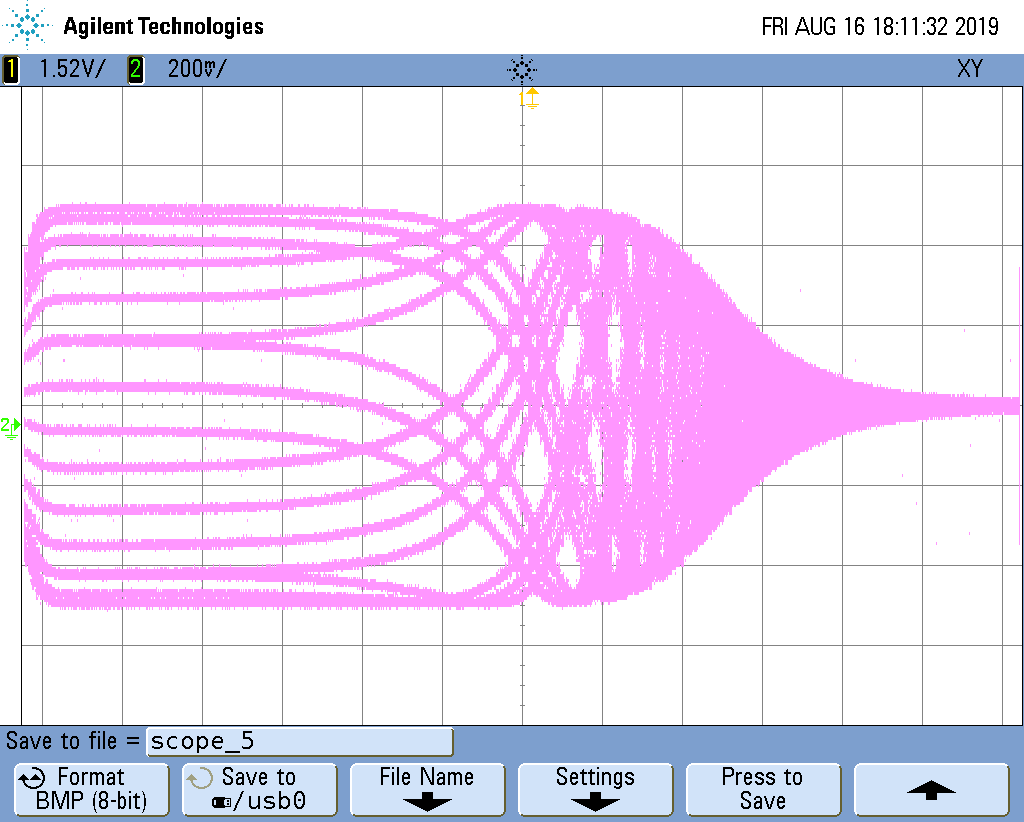
\includegraphics[width=0.8\textwidth,trim={0.5cm 5cm  1 5cm},clip]{ej3xy.png}
	\caption{Medición de la respuesta en frecuencia del circuito de la figura \ref{figure:circuito_Pasa_bajos} utilizando el método XY y dos generadores.} 
	\label{graf:osci_freq_alta}
\end{figure}

\subsubsection*{Modo Normal}
Por otro lado, se utilizó el modo normal, disparado acordemente, es decir, utilizando un solo generador de funciones.
\begin{figure}[H]
	\centering
	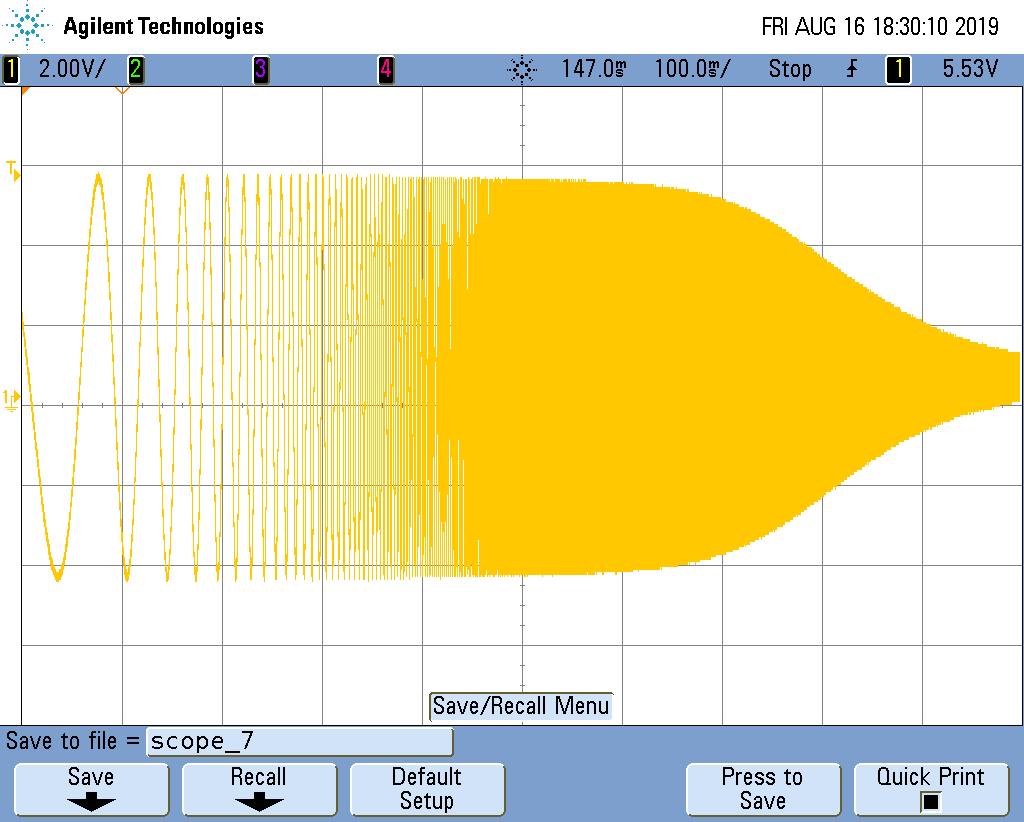
\includegraphics[width=0.8\textwidth,trim={0.6cm 7cm  1 5cm},clip]{ej3normal.png}
	\caption{Medición de la respuesta en frecuencia del circuito de la figura \ref{figure:circuito_Pasa_bajos} utilizando el modo normal del trigger.} 
	\label{graf:ej3modonormal}
\end{figure}
Se utilizó un barrido en frecuencia desde $100 \ mHz$ hasta $100 \ kHz$, en un período total de 2 segundos con una amplitud de 5 volt pico a pico. Para lograr visualizar la mayor parte de la respuesta en frecuencia, se utilizó el modo Single del osciloscopio, con el trigger en una amplitud igual a la de la salida al comienzo del barrido. Se observa que este modo de usar el osciloscopio puede ser una forma fácil de visualizar a la respuesta en frecuencia de un circuito de forma rápida y muy aproximada. No se presentaron mayores dificultades a la hora de realizar la medición.

\break

\subsection*{Respuesta en Frecuencia del Osciloscopio}
Finalmente, se midió la respuesta en frecuencia del Agilent DSO6014A del laboratorio, activando los filtros AC y BW. Se esperaba, según la teoría, que la respuesta sea similar a la de un filtro pasa-banda, atenuando las frecuencias muy bajas y muy altas. Esto es, realizando a priori la suposición de que el generador de funciones nos proporcionará una amplitud de señal constante a todas las frecuencias.

Para realizar la medición, se conectó el osciloscopio con las puntas en x10 previamente calibradas, se activaron los filtros y se conectaron las puntas del osciloscopio a la salida de un generador de funciones con una señal sinusoidal de 20 voltios pico a pico para minimizar la lectura de ruido. Se comenzó a medir desde una frecuencia muy pequeña, de $10 \ mHz$, obteniendo la ganancia de tensión midiendo pico a pico la señal del osciloscopio y dividiéndola por el valor mostrado en el generador. Se finalizó la medición con la mayor frecuencia que admite el generador usado, de $15 \ MHz$.

Finalmente, se utilizó python para graficar la respuesta en frecuencia en amplitud del osciloscopio con los filtros BW y AC, observado en la figura \ref{graf:resp_freq_osci}.

\begin{figure}[H]
	\centering
	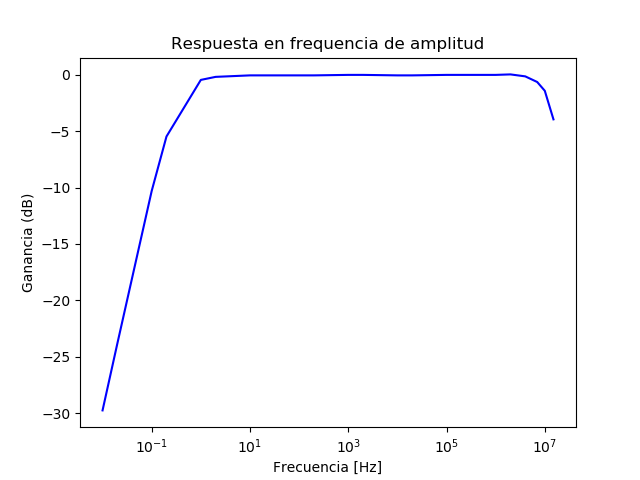
\includegraphics[width=0.8\textwidth]{resp_freq_osci.png}
	\caption{Gráfico de la respuesta en frecuencia del DSO6014A con los filtros BW y AC.} 
	\label{graf:resp_freq_osci}
\end{figure}

No habiendo quedado conforme con el generador utilizado y su rango de frecuencias, se decidió volver a realizar la medición con el mismo osciloscopio pero utilizando otro generador de funciones cuyo límite de frecuencia era de $50 \ MHz$. Se repitieron todos los pasos anteriores para realizar la medición, sin embargo, se detectaron comportamientos anómalos en las frecuencias medias que en la medición anterior no se habían detectado. La ganancia medida para estos valores de frecuencia eran de alrededor de los $4 \ dB$.

Tras esta medición, se decidió comenzar con las mediciones de nuevo minimizando el error cometido. Se utilizaron dos puntas de osciloscopio, ambas para medir la salida del generador pero activando los filtros solo en una de ellas. Se calculó la ganancia de tensión y fase entre las dos lecturas. Sin embargo, se concluyó que el osciloscopio estaba trabajando de forma no óptima o errónea, ya que las mediciones anteriores de amplificación volvieron a surgir, pero tras configurar nuevamente el menu de medición del osciloscopio, la medición cambió a un resultado mas sensato. Se decidió terminar la medición de todos modos y presentar la siguiente transferencia de tensión junto a la fase en función de la frecuencia.

\begin{figure}[H]
	\centering
	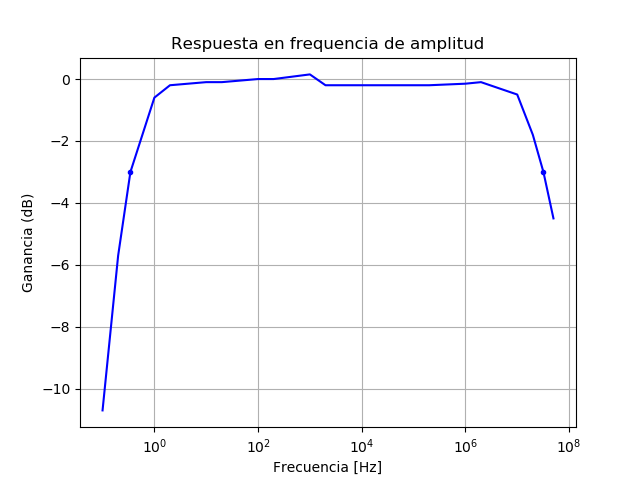
\includegraphics[width=0.8\textwidth]{resp_freq_osci1.png}
	\caption{Gráfico de la respuesta en frecuencia de amplitud del DSO6014A con los filtros BW y AC segunda medición.}  
	\label{graf:resp_freq_osci1}
\end{figure}

\begin{figure}[H]
	\centering
	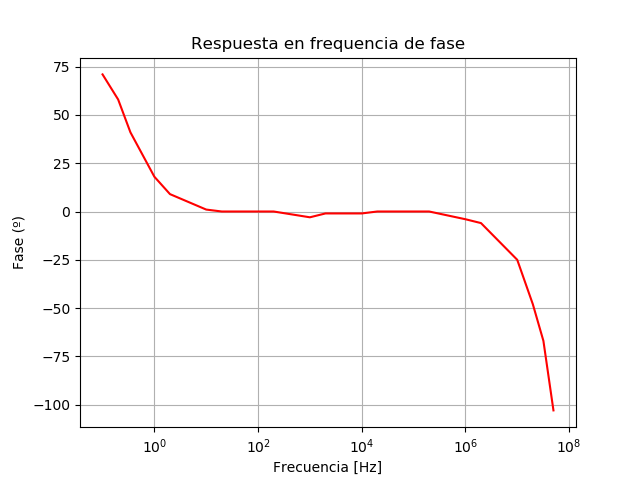
\includegraphics[width=0.8\textwidth]{resp_freq_osci2.png}
	\caption{Gráfico de la respuesta en frecuencia de fase del DSO6014A con los filtros BW y AC segunda medición.} 
	\label{graf:resp_freq_osci2}
\end{figure}

Se puede observar que en la práctica la respuesta en frecuencia del osciloscopio resulta ser un pasabanda, que atenua frecuencias menores a $\approx 1 \ Hz$ y mayores a $\approx 1 \ MHz$. Estos resultados verifican la suposición hecha con ayuda de los conocimientos de la teoría. Se observa también que los filtros utilizados limitan al osciloscopio en ancho de banda significativamente, ya que según el fabricante la frecuencia a la que se atenúan las señales por $3 \ dB$ es de $100 \ MHz$, mientras que en la figura \ref{graf:resp_freq_osci1} puede verse que esa frecuencia es de $32 \ MHz$.

Si se comparan los datos obtenidos con los datos del fabricante:
\begin{center}
BANDWIDTH $\rightarrow$ MSO/DSO601xA: DC to 100 MHz\\
AC-COUPLED $\rightarrow$ MSO/DSO601xA: 3.5 Hz to 100 MHz\\
BW LIMIT $\rightarrow$ MSO/DSO601xA: 20 MHz selectable\\
\end{center}

Se presentan diferencias grandes respecto a la práctica, ya que la frecuencia de corte medida para las frecuencias muy bajas es de $345 \ mHz$ mientras que la frecuencia de corte provista por el fabricante es de $3.5 \ Hz$. No se logró hallar una razón que logre explicar esta discrepancia, ya que mismas mediciones realizadas por otras personas en distintos momentos reportaron la misma frecuencia de corte. Se concluye que la hoja de datos del osciloscopio debe tener una falla.

Respecto a la frecuencia de corte para las frecuencias altas, se encontró que esta se situaba a una frecuencia de $32 \ MHz$, también distinta a la provista por el fabricante. Tampoco se logró encontrar alguna explicación a esta discrepancia, aunque es imposible descartar la cantidad de problemas que hubo con el osciloscopio utilizado como fuente de error en la medición.

\end{document}
